\section{EKLER}

FaceScan AI bulut projesine ait doğrulanabilir dijital kaynak bağlantıları ve erişim adresleri aşağıda sunulmuştur:

\subsection{Dijital Kaynak Bağlantıları}
\begin{itemize}
    \item \textbf{Canlı Bulut Dağıtım Adresi:} \url{https://face-diagnose-app.vercel.app}
    \item \textbf{Bulut Sunucusundaki Android APK İndirme Bağlantısı:} \url{https://face-diagnose-app.vercel.app/facescan-ai.apk}
    \item \textbf{Bulut Sunucusundaki MobSF PDF Güvenlik Raporu:} \url{https://face-diagnose-app.vercel.app/mobsf-report.pdf}
    \item \textbf{GitHub Kaynak Kod Deposu:} \url{https://github.com/ozgursekmenn/face-scan-ai}
\end{itemize}

\subsection{Sistem Dağıtım Ekran Görüntüleri}
Uygulama arayüzünün bulut üzerindeki responsive görünümü, Vercel paneli dağıtım kayıtları ve MobSF analiz sonuç detayları projenin canlı web adresinde yer alan "Hakkında" (Info) sekmesi altında görüntülenebilmektedir.

Aşağıdaki Şekil \ref{fig:bulut_ekler_genel1} ve Şekil \ref{fig:bulut_ekler_genel2}'de bulut dağıtımı tamamlanmış olan uygulamanın canlı ve mobil entegrasyon arayüzlerinden görünümler bir arada sunulmaktadır.

\begin{figure}[h!]
    \centering
    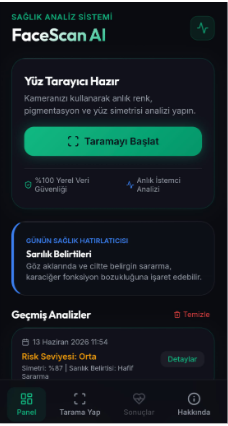
\includegraphics[width=0.30\linewidth]{sekil2_dashboard.png}
    \hspace{0.5cm}
    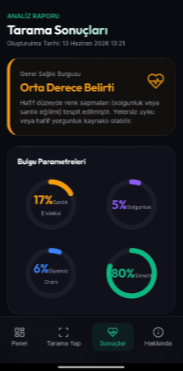
\includegraphics[width=0.30\linewidth]{sekil5_sonuclar.png}
    \hspace{0.5cm}
    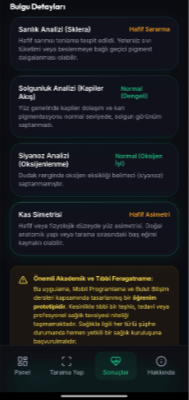
\includegraphics[width=0.30\linewidth]{sekil6_detaylar.png}
    \caption{FaceScan AI Canlı Sistem Arayüzleri -- Sol: Dashboard, Orta: Sonuç Ekranı, Sağ: Bulgu Detayları}
    \label{fig:bulut_ekler_genel1}
\end{figure}

\begin{figure}[h!]
    \centering
    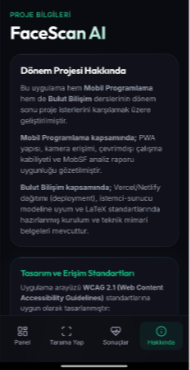
\includegraphics[width=0.30\linewidth]{sekil7_hakkinda_1.png}
    \hspace{0.5cm}
    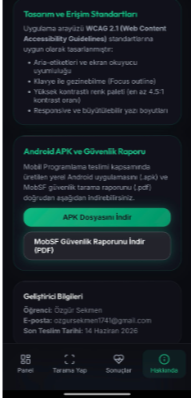
\includegraphics[width=0.30\linewidth]{sekil8_hakkinda_2.png}
    \hspace{0.5cm}
    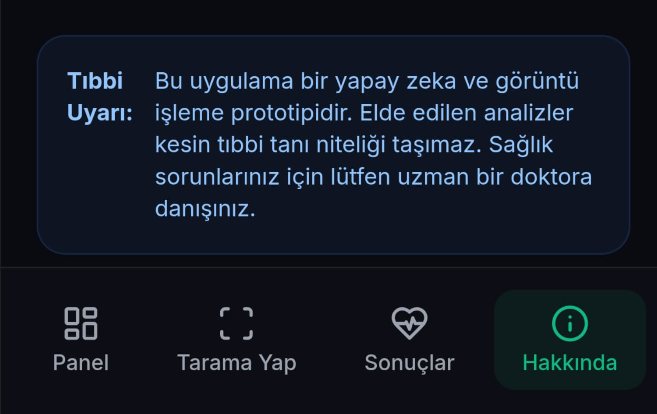
\includegraphics[width=0.30\linewidth]{sekil9_tibbi_uyari.png}
    \caption{FaceScan AI Hakkında ve Güvenlik/Tıbbi Uyarı Ekranları -- Sol: Proje Bilgileri, Orta: APK/Rapor İndirme Sekmesi, Sağ: Tıbbi Sorumluluk Reddi Bildirimi}
    \label{fig:bulut_ekler_genel2}
\end{figure}

